\appendices

\ifexpDist
\section{Distribution of the current magnitudes}\label{app:dist}
The leakage currents span many decades (Table~\ref{tab:dist}). The ON datasets are concentrated at $10^{-5}$--$10^{-4}$\,A (44.7\,\% of the NMOS ON and 46.7\,\% of the PMOS ON rows have $|i_s|$ in that decade). NMOS OFF is concentrated between $10^{-12}$ and $10^{-10}$\,A (67.7\,\% of the rows); PMOS OFF is spread almost evenly over the decades from below $10^{-15}$ to $10^{-11}$\,A (12--18\,\% per decade), and 63.5\,\% of its rows are below $10^{-12}$\,A.
Small currents inside the ON datasets come from weakly driven devices, not from the corner with both terminals at $V_{DD}$: of the 162 PMOS ON rows with $|i_d|$ between $10^{-13}$ and $10^{-11}$\,A, all have the higher of $V_d,V_s$ below $|V_{th0}|$ (subthreshold operation), none has both terminals within 100\,mV of $V_{DD}$, and only 99 of the 10,000 rows (0.99\,\%) have both terminals that close to $V_{DD}$.
% src: results/analysis/report_numbers/current_magnitude_distribution_pct.csv, report_data_stats.txt, validation_checks/pmos_on_small_currents2.txt
\begin{table}[t]
\caption{Distribution of $|i_s|$ in percent of the 10,000 rows per case.}
\label{tab:dist}
\centering\footnotesize
\setlength{\tabcolsep}{3pt}
\fitcol{% src: results/analysis/report_numbers/current_magnitude_distribution_pct.csv
\begin{tabular}{lrrrr}
\toprule
$|i_s|$ range (A) & NMOS ON & NMOS OFF & PMOS ON & PMOS OFF \\
\midrule
$<$1e-15 & 0.00 & 0.02 & 0.02 & 17.71 \\
1e-15--1e-14 & 0.01 & 0.11 & 0.06 & 15.94 \\
1e-14--1e-13 & 0.16 & 1.11 & 0.24 & 14.64 \\
1e-13--1e-12 & 0.34 & 9.52 & 0.59 & 15.23 \\
1e-12--1e-11 & 0.79 & 32.71 & 1.08 & 12.62 \\
1e-11--1e-10 & 1.60 & 35.03 & 1.96 & 9.90 \\
1e-10--1e-9 & 2.56 & 14.24 & 2.72 & 7.65 \\
1e-9--1e-8 & 3.58 & 5.67 & 3.62 & 4.55 \\
1e-8--1e-7 & 4.93 & 1.47 & 5.15 & 1.59 \\
1e-7--1e-6 & 7.37 & 0.12 & 8.33 & 0.17 \\
1e-6--1e-5 & 14.34 & 0.00 & 19.72 & 0.00 \\
1e-5--1e-4 & 44.66 & 0.00 & 46.69 & 0.00 \\
$>$=1e-4 & 19.66 & 0.00 & 9.82 & 0.00 \\
\bottomrule
\end{tabular}
}
\end{table}
\fi

\ifexpFamilies
\section{Gate accuracy per model family (for comparison only)}\label{app:family}
To see how much the model family matters at gate level we evaluated each family on its own for all four transistor cases (Table~\ref{tab:family}). \emph{These numbers are for comparison only; they were not used to choose the final models}, which were chosen on validation data only. The ResNet, which is among the best on the validation set, fails on NAND2 \texttt{00} (51.0\,\% mean accuracy with the 80:10:10 models, 24.6\,\% with the 70:15:15 models) because of its PMOS ON model: that case has the smallest leakage of the NAND2 cases (median $\SI{5.4e-10}{\ampere}$), and the gate currents of the two ON PMOS, which the super-node sum keeps, dominate it. GPR is accurate for the ON cases and is used there in the final set.
% src: results/analysis/report_numbers/family_gate_accuracy.csv, results/partB/gate_results.csv
\begin{table}[t]
\caption{One model family for all four cases, gate and circuit mean accuracy (\%); for comparison only, not used for selection.}
\label{tab:family}
\centering\footnotesize
\setlength{\tabcolsep}{2.5pt}
\fitcol{% src: results/analysis/report_numbers/family_gate_accuracy.csv
\begin{tabular}{llrrrr}
\toprule
Split & Family & Part B mean acc. & NAND2 00 & NAND2 all & Part C mean acc. \\
\midrule
80:10:10 & GPR & 94.48 & 96.15 & 94.93 & 93.19 \\
 & Hybrid & 96.96 & 79.78 & 93.77 & 97.60 \\
 & ResNet & 96.17 & 51.02 & 86.86 & 98.90 \\
 & PINN & 96.42 & 82.96 & 94.12 & 97.66 \\
\midrule
70:15:15 & GPR & 93.07 & 95.59 & 94.07 & 91.03 \\
 & Hybrid & 97.14 & 94.00 & 96.90 & 96.74 \\
 & ResNet & 94.39 & 24.64 & 79.98 & 98.81 \\
 & Components MLP & 95.47 & 74.95 & 91.69 & 96.27 \\
\bottomrule
\end{tabular}
}
\end{table}
\fi

\section{Predicted versus SPICE currents of the chosen models}\label{app:parity}
\begin{figure*}[t]
\centering
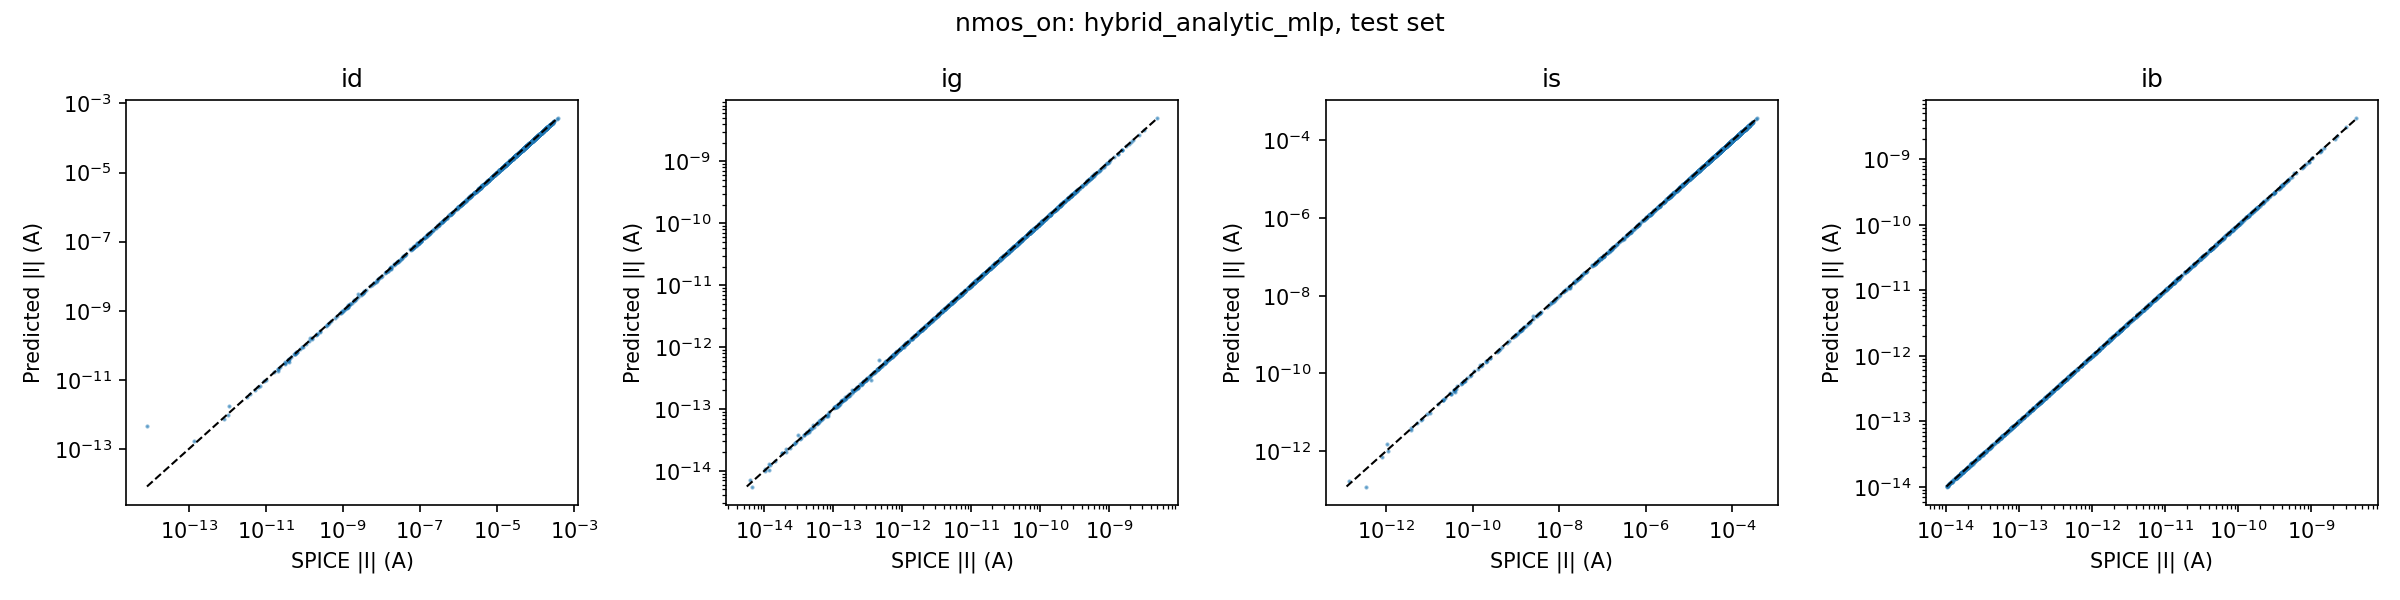
\includegraphics[width=0.78\textwidth]{figures/parity_nmos_on.png}\\[1mm]
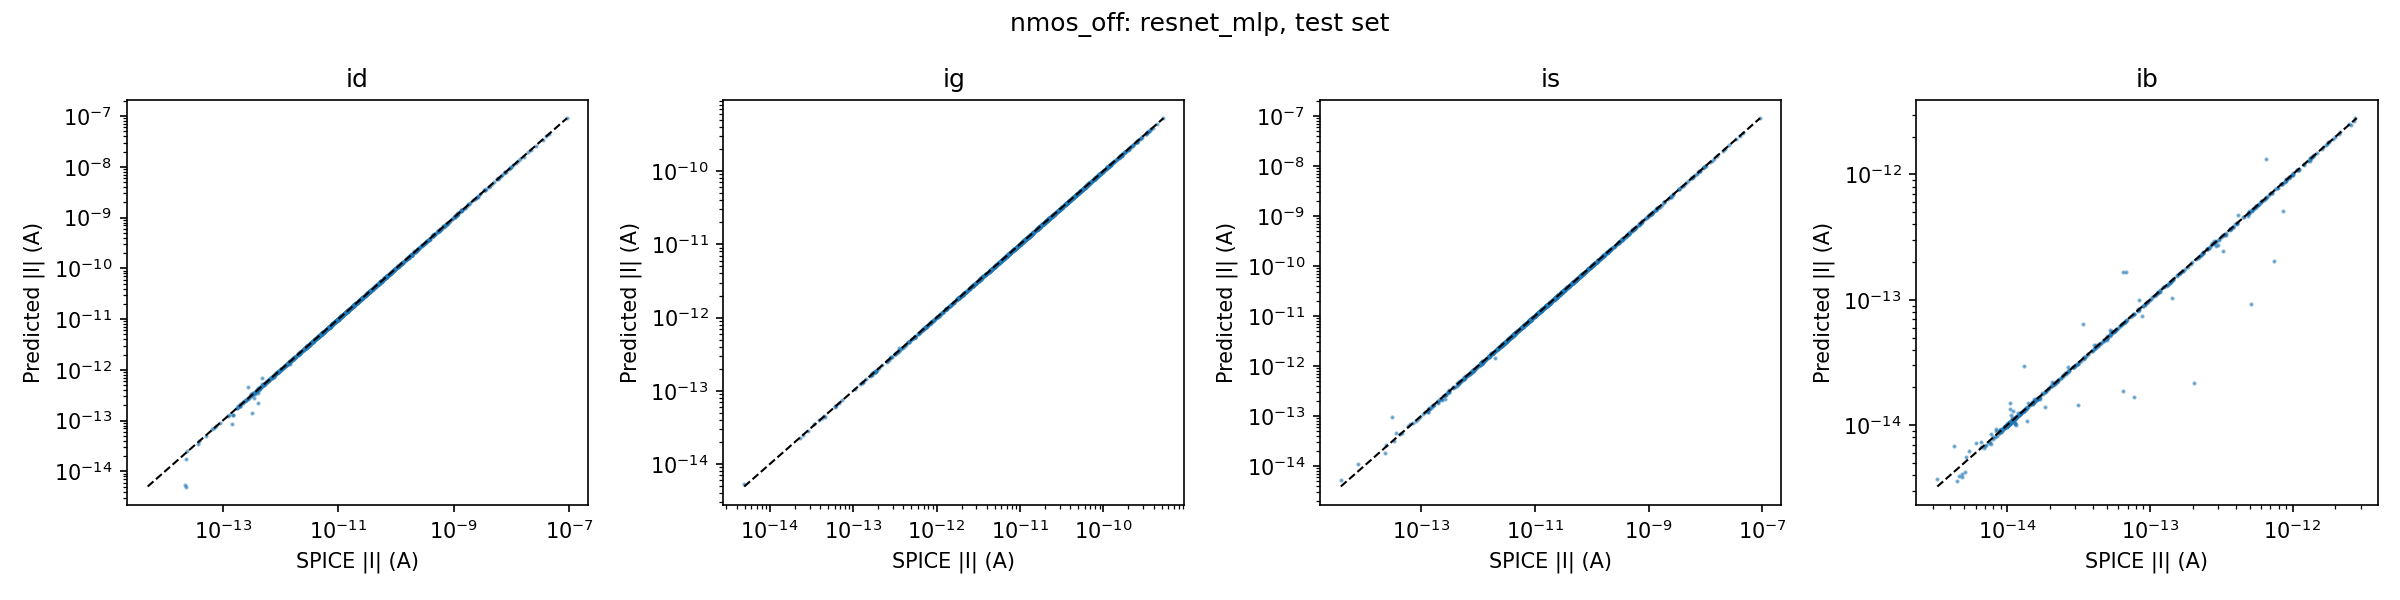
\includegraphics[width=0.78\textwidth]{figures/parity_nmos_off.png}\\[1mm]
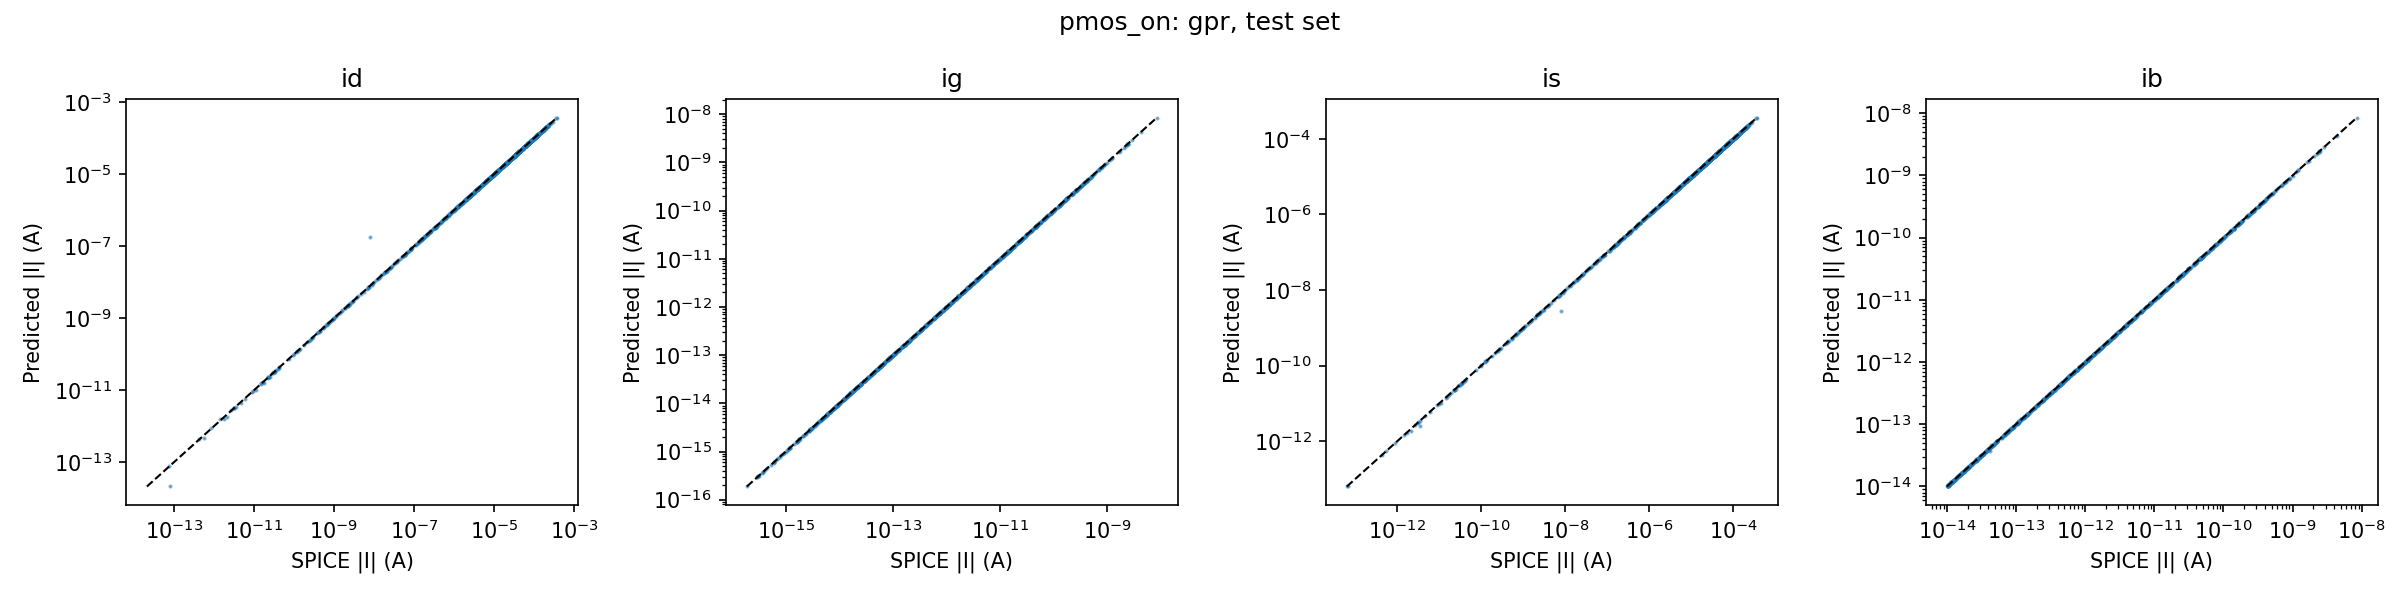
\includegraphics[width=0.78\textwidth]{figures/parity_pmos_on.png}\\[1mm]
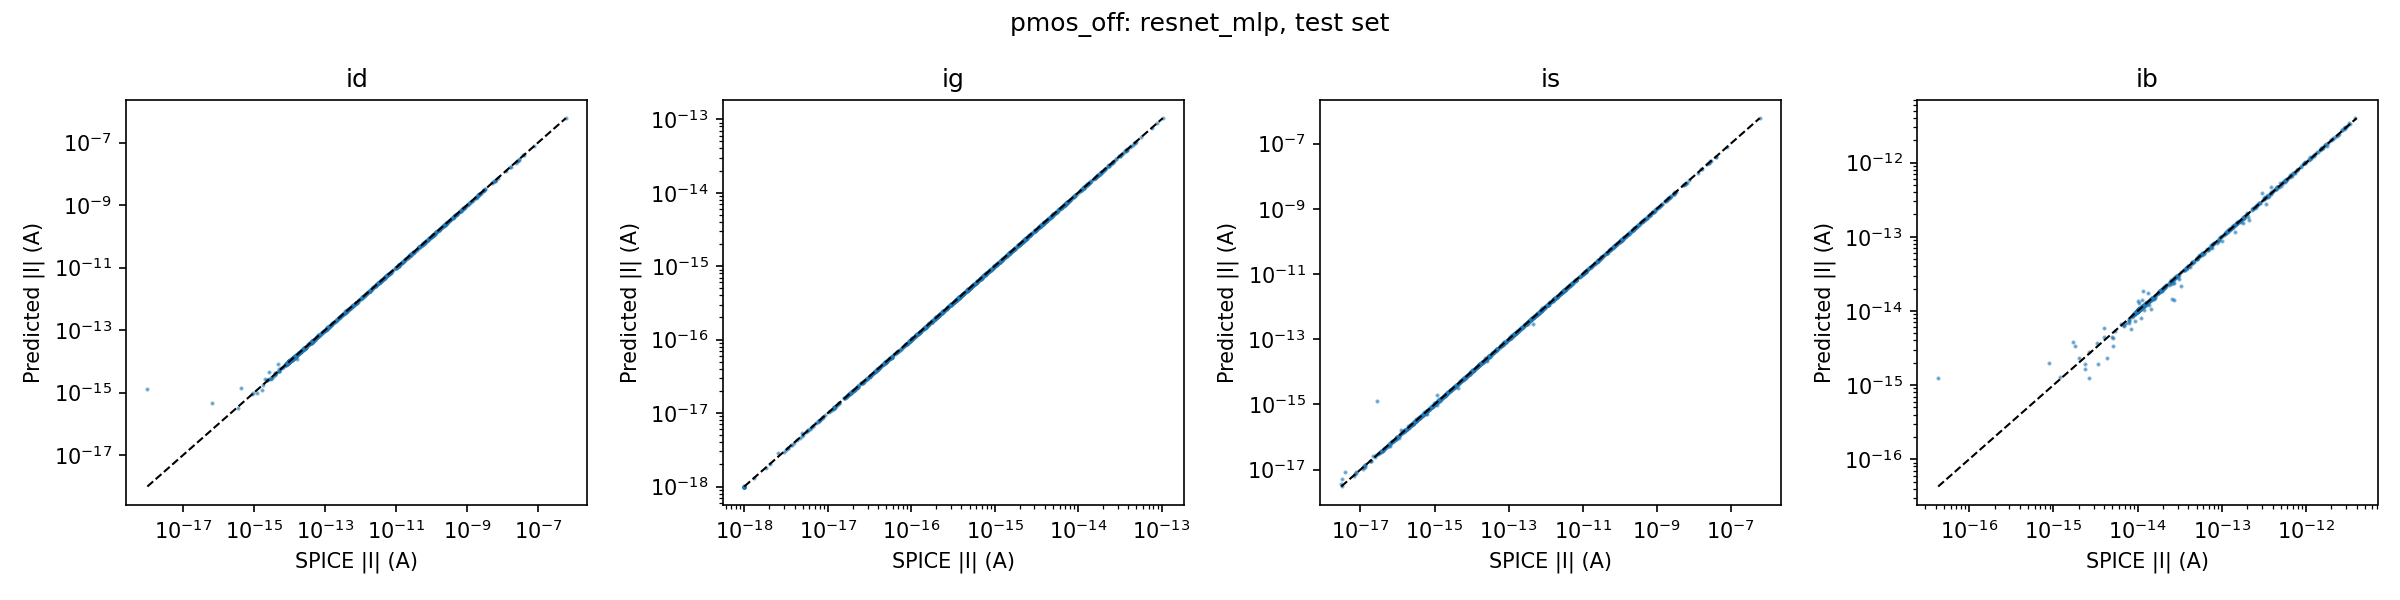
\includegraphics[width=0.78\textwidth]{figures/parity_pmos_off.png}
\caption{Chosen models on the test set: predicted versus SPICE $|I|$ for $i_d$, $i_g$, $i_s$, $i_b$ (log axes, dashed: prediction $=$ SPICE). From top: NMOS ON (hybrid), NMOS OFF (ResNet), PMOS ON (GPR), PMOS OFF (ResNet).}
\label{fig:parity}
% src: results/partA/parity_<case>.png
\end{figure*}
